\documentclass[12pt,a4paper]{article}
\usepackage{setspace}
\onehalfspacing
\usepackage{hyperref}
\hypersetup{
	colorlinks,
	citecolor=black,
	filecolor=black,
	linkcolor=black,
	urlcolor=blue
}
\usepackage[]{times}
\usepackage[latin1]{inputenc}
\usepackage{amsmath}
\usepackage{amsfonts}
\usepackage{amssymb}
\usepackage{makeidx}
\usepackage{graphicx}
\usepackage{multirow} % Required for multirows

\begin{document}
	
	\title{Web Security Application}
	\author{Becker, Joshua\\ Okereke, Uchechukwu Okpo\\ Shama, Muthuraman Venkatesan\\ Ulbrich, Damian}
	\date{\today}
	\maketitle
	\thispagestyle{empty}
	\clearpage
	
	
	\tableofcontents
	\thispagestyle{empty}
	\clearpage
	\pagenumbering{arabic} 
	\section{Introduction}
	
	
	\begin{flushleft}
	Since the creation of the Internet, the world has seen it evolve with lots of practical applications. These include things like eCommerce, Instant Messaging, Video Streaming services and the likes. With this evolution and advancements, there has also been a rise in misuse and security concerns regarding identity theft, private data leaks etc.
	
		
	One subset of eCommerce that is ever so popular is Online shopping, allowing consumers to buy goods or order services directly from a seller over the Internet. Hence, the element of security for user details is crucial.
	
	
	In this project, we were tasked to create a simple eCommerce site called Webshop. We look to see how a user can interact with the online store and be able to make purchases with or without registering on the site while being safeguarded against security attacks. This report, documents the required specifications of the project, alongside how the requirements were implemented. Also, the challenges encountered during the course of the project.
	
		
	\section{Architecture}
	
	Because this was a test project, a "One-Tier Architecture" approach was taken. This involves putting all of the required components for a software application or technology on a single server or platform [1]. In future, this can be scaled to an "N-Tier Architecture".  As seen in figure 1, the 1-tier architecture consist of three parts: Presentation layer, Application layer and the Database layer. To achieve this XAMP (Cross-Platform, Apache, MariaDB, PHP) was used. 
	\begin{figure}[h]
			\begin{center}
				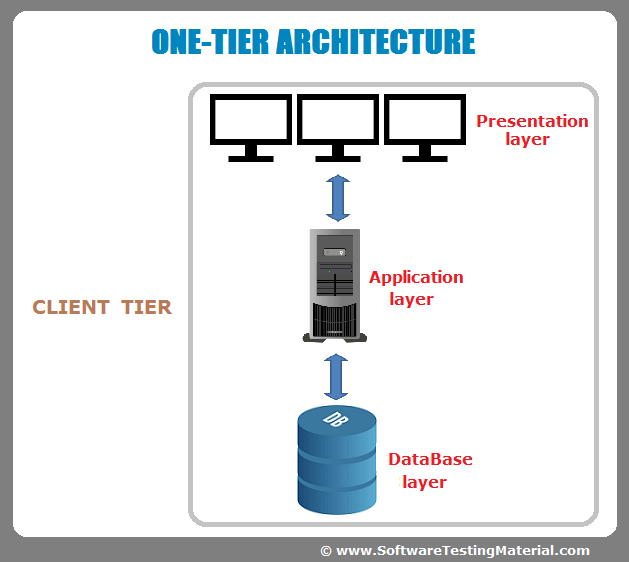
\includegraphics[scale = 0.3]{one-tier-software-architecture}
			
			\caption{One-Tier Architecture}
			
			\end{center}
		\end{figure}
		
	\begin{itemize}
		\item 	Presentation Layer: This is usually referred to as the application frontend. This is the layer a user or client interacts with. HTML, CSS and a bit of Javascript was used to achieve this.
		
		\item Application Layer: Usually referred to as the backend of an application. This contains all the logic needed for the application to function properly from structure to security of the application. Making this the major focus of this project and PHP (Hypertext Preprocessor) was used here.
		
		\item Database Layer: This is where all user and admin data were stored. MySQL which is an open-source relational database management system, was used to create, store, read and update both user and admin data.
	\end{itemize}
	To download and install this project, one must first install \textbf{\textit{XAMPP}} and clone the git repository (https://github.com/muthuramansv/webappsecurity.git) into the \textbf{\textit{htdocs}} folder. Start up XAMP, connect the database and run "localhost/webappsecurity/Integration/index.php".
	
	
	
	\section{Features}
	The sole criteria for this project was security based and the following features were required.
	\begin{itemize}
		\item \textbf{Secure Session Handling:} A web session is a sequence of network HTTP request and response transactions associated to the same user [2]. 
		Web applications can keep track of both anonymous and authenticated users via a session ID, usually called a Token. A cookie is among the many forms of managing or handling a session. Since authenticated sessions contain lots of private information, they need to be protected from theft attacks which could lead to impersonation of a legitimate user. In other to guard against this, tokens need to be given an expiration time, rendering the session invalid and useless if stolen.
		
		\item \textbf{Secure Password Storage:} To prevent theft of user credentials, passwords need to be stored securely in the database. One way of achieving this is to never store the password as plaintext, instead salt and hash the user password before storing it in the database. There are several cryptographic algorithms available for this but not all suitable to prevent brute force attacks or rainbow tables. In this project the PHP password\_hash() function was used. It is a strong one-way algorithm, which automatically salts and hashes the inputed plaintext. The output (figure 2) can then be stored in the database.
		\begin{figure}[h]
			\begin{center}
				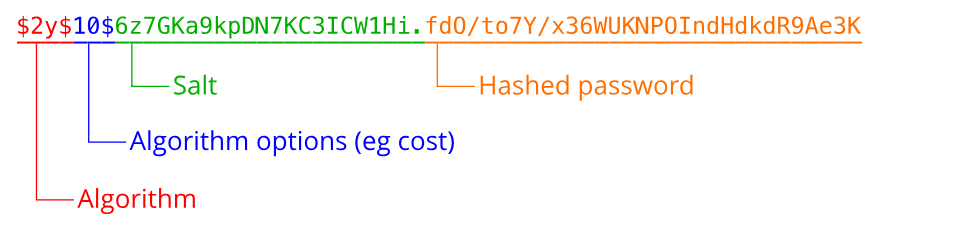
\includegraphics [scale = 0.3] {algo}
				\caption{Hashed Password Sample}
				Source: Safe Password Hashing, PHP Documentation
			\end{center}
		\end{figure}
		
		\textbf{\item Cross-Site Request Forgery Handling:} This occurs when an attacker uses a malicious web site, email, blog, instant message, or program to cause a user?s web browser to perform an unwanted action on a trusted site for which the user is currently authenticated [3]. In order to handle this attack a random token was generated and verified alongside.
				
		\textbf{\item Cross-Site Scripting Handling:} This involves the insertion of malicious scripts into benign and trusted websites[4]. The attacker sends malicious code which is then used to steal a legitimate user cookie by redirecting the user to a different site or through popups. The easiest way of preventing this attack was to escape all untrusted data before echoing it out to the user.
		
		\textbf{\item SQL-Injection Handling:} This consists of putting a SQL query via the input data from the client to the web application[5]. To prevent this we made use of prepared statements with parameterized queries, which ensures an attacker cannot change the database query even when another SQL command is inserted by the attacker.
	\end{itemize}
	
		
	\section{Tools Used}
	Teamwork and collaboration is usually a tricky subject, but thanks to certain technologies that has helped to ease this burden. The following are a list of tools we worked with for both collaboration and application building:
	\begin{itemize}
		\item \textbf{Git:} Git is a version control system that helps track changes in project files. This really helps when coding on different platforms and machines. Source codes can be managed efficiently, generating less bugs.
		
		\item \textbf{Trello:} This is a web-based tool which helps with project management. Trello allowed us to take an Agile approach towards completion of this project.
		
		\item \textbf{WhatsApp:} A bit strange, but yes, WhatsApp was our default communication tool. Group meet-ups and questions were conveyed through this medium.
			
	\end{itemize}
	
	
	\section {Team Matrix}
	\begin{tabular}{|l|c|c|c|c|}
		\hline
		 & Becker & Okereke & Shama & Ulbrich \\ \hline
		 Project Planning & x & x & x & x \\ \hline
		 Database Design & x &  &  & x \\ \hline
		 XSS Handling &  & x &  &  \\ \hline
		 CSRF Handling &  &  &  &  \\ \hline
		 Sessions Management & x &  &  &  \\ \hline
		 Frontend Design &  &  & x &  \\ \hline
		 SQL Injection Handling &  &  &  & x \\ \hline
		 %Project Planning & x & x & x & x \\ \hline
		 %Project Planning & x & x & x & x \\ \hline
		 %Project Planning & x & x & x & x \\ \hline
		 %Project Planning & x & x & x & x \\ \hline
		 Documentation &  & x &  &  \\ \hline
	\end{tabular}
	
	\end{flushleft}
	
	
	
	
	\section{Challenges and Lessons Learnt}
	\subsection{TEAM CHALLENGES}
	\begin{flushleft}
	
		We were faced with the following challenges:
		\begin{itemize}
			\item \textbf{Time:} We had to figure out time to gather so we could work together since some of us didn?t have prior
			experience in programming.
			\item \textbf{Git:} Working with Git can always be tricky especially when merge conflicts arise. Lucky for us we were able to solve them.
			\item \textbf{Secure Logic:} On paper it sounds simple, but figuring out how to come up with a secure logic and avoid different security task was tough.
		\end{itemize}
		
	\end{flushleft}
	
	
	\subsection{LESSONS LEARNT}
	\begin{flushleft}
		The following are a list of things learnt during the course of this project.
		\begin{itemize}
		\item \textbf{Coding Skills:} Every team member learnt a lot about PHP, MySQL and how various functions works. Since we developed a XAMPP stack application, we developed skills from frontend to backend. Also worth noting is it never got easier we just got better.
		\item \textbf{Knowledge:} There is a lot of knowledge passed across to us during the lecture time from the first lecture to the end with practical examples.
		\item \textbf{Team work:} This is one of the key skills that was learn in this course, we were taught how to build and work as a
		team which helps us in our daily lives.
		\item \textbf{Feedback:} We learned how to give and receive feedback in a friendly and professional way which helped to achieve the goal of delivering a successful project.
		\end{itemize}
	\end{flushleft}
	
	\section{REFERENCES}
	
	\begin{enumerate}
		\item Software Architecture: One-Tier, \textit{https://www.techopedia.com/definition/17374/one-tier-architecture}
		\item Session Management Cheat Sheet, \textit{https://www.owasp.org/index.php/Session\_Management\_Cheat\_Sheet}
		\item Cross-Site Request Forgery (CSRF) Prevention Cheat Sheet, \textit{https://www.owasp.org/index.php/Cross-Site\_Request\_Forgery\_(CSRF)\_Prevention\_Cheat\_Sheet}
		\item Cross-site Scripting, https://www.owasp.org/index.php/Cross-site\_Scripting\_(XSS)
		\item SQL Injection, https://www.owasp.org/index.php/SQL\_Injection
	\end{enumerate}
	
		
	
\end{document}